
% Default to the notebook output style

    


% Inherit from the specified cell style.




    
\documentclass[11pt]{article}

    
    
    \usepackage[T1]{fontenc}
    % Nicer default font (+ math font) than Computer Modern for most use cases
    \usepackage{mathpazo}

    % Basic figure setup, for now with no caption control since it's done
    % automatically by Pandoc (which extracts ![](path) syntax from Markdown).
    \usepackage{graphicx}
    % We will generate all images so they have a width \maxwidth. This means
    % that they will get their normal width if they fit onto the page, but
    % are scaled down if they would overflow the margins.
    \makeatletter
    \def\maxwidth{\ifdim\Gin@nat@width>\linewidth\linewidth
    \else\Gin@nat@width\fi}
    \makeatother
    \let\Oldincludegraphics\includegraphics
    % Set max figure width to be 80% of text width, for now hardcoded.
    \renewcommand{\includegraphics}[1]{\Oldincludegraphics[width=.8\maxwidth]{#1}}
    % Ensure that by default, figures have no caption (until we provide a
    % proper Figure object with a Caption API and a way to capture that
    % in the conversion process - todo).
    \usepackage{caption}
    \DeclareCaptionLabelFormat{nolabel}{}
    \captionsetup{labelformat=nolabel}

    \usepackage{adjustbox} % Used to constrain images to a maximum size 
    \usepackage{xcolor} % Allow colors to be defined
    \usepackage{enumerate} % Needed for markdown enumerations to work
    \usepackage{geometry} % Used to adjust the document margins
    \usepackage{amsmath} % Equations
    \usepackage{amssymb} % Equations
    \usepackage{textcomp} % defines textquotesingle
    % Hack from http://tex.stackexchange.com/a/47451/13684:
    \AtBeginDocument{%
        \def\PYZsq{\textquotesingle}% Upright quotes in Pygmentized code
    }
    \usepackage{upquote} % Upright quotes for verbatim code
    \usepackage{eurosym} % defines \euro
    \usepackage[mathletters]{ucs} % Extended unicode (utf-8) support
    \usepackage[utf8x]{inputenc} % Allow utf-8 characters in the tex document
    \usepackage{fancyvrb} % verbatim replacement that allows latex
    \usepackage{grffile} % extends the file name processing of package graphics 
                         % to support a larger range 
    % The hyperref package gives us a pdf with properly built
    % internal navigation ('pdf bookmarks' for the table of contents,
    % internal cross-reference links, web links for URLs, etc.)
    \usepackage{hyperref}
    \usepackage{longtable} % longtable support required by pandoc >1.10
    \usepackage{booktabs}  % table support for pandoc > 1.12.2
    \usepackage[inline]{enumitem} % IRkernel/repr support (it uses the enumerate* environment)
    \usepackage[normalem]{ulem} % ulem is needed to support strikethroughs (\sout)
                                % normalem makes italics be italics, not underlines
    

    
    
    % Colors for the hyperref package
    \definecolor{urlcolor}{rgb}{0,.145,.698}
    \definecolor{linkcolor}{rgb}{.71,0.21,0.01}
    \definecolor{citecolor}{rgb}{.12,.54,.11}

    % ANSI colors
    \definecolor{ansi-black}{HTML}{3E424D}
    \definecolor{ansi-black-intense}{HTML}{282C36}
    \definecolor{ansi-red}{HTML}{E75C58}
    \definecolor{ansi-red-intense}{HTML}{B22B31}
    \definecolor{ansi-green}{HTML}{00A250}
    \definecolor{ansi-green-intense}{HTML}{007427}
    \definecolor{ansi-yellow}{HTML}{DDB62B}
    \definecolor{ansi-yellow-intense}{HTML}{B27D12}
    \definecolor{ansi-blue}{HTML}{208FFB}
    \definecolor{ansi-blue-intense}{HTML}{0065CA}
    \definecolor{ansi-magenta}{HTML}{D160C4}
    \definecolor{ansi-magenta-intense}{HTML}{A03196}
    \definecolor{ansi-cyan}{HTML}{60C6C8}
    \definecolor{ansi-cyan-intense}{HTML}{258F8F}
    \definecolor{ansi-white}{HTML}{C5C1B4}
    \definecolor{ansi-white-intense}{HTML}{A1A6B2}

    % commands and environments needed by pandoc snippets
    % extracted from the output of `pandoc -s`
    \providecommand{\tightlist}{%
      \setlength{\itemsep}{0pt}\setlength{\parskip}{0pt}}
    \DefineVerbatimEnvironment{Highlighting}{Verbatim}{commandchars=\\\{\}}
    % Add ',fontsize=\small' for more characters per line
    \newenvironment{Shaded}{}{}
    \newcommand{\KeywordTok}[1]{\textcolor[rgb]{0.00,0.44,0.13}{\textbf{{#1}}}}
    \newcommand{\DataTypeTok}[1]{\textcolor[rgb]{0.56,0.13,0.00}{{#1}}}
    \newcommand{\DecValTok}[1]{\textcolor[rgb]{0.25,0.63,0.44}{{#1}}}
    \newcommand{\BaseNTok}[1]{\textcolor[rgb]{0.25,0.63,0.44}{{#1}}}
    \newcommand{\FloatTok}[1]{\textcolor[rgb]{0.25,0.63,0.44}{{#1}}}
    \newcommand{\CharTok}[1]{\textcolor[rgb]{0.25,0.44,0.63}{{#1}}}
    \newcommand{\StringTok}[1]{\textcolor[rgb]{0.25,0.44,0.63}{{#1}}}
    \newcommand{\CommentTok}[1]{\textcolor[rgb]{0.38,0.63,0.69}{\textit{{#1}}}}
    \newcommand{\OtherTok}[1]{\textcolor[rgb]{0.00,0.44,0.13}{{#1}}}
    \newcommand{\AlertTok}[1]{\textcolor[rgb]{1.00,0.00,0.00}{\textbf{{#1}}}}
    \newcommand{\FunctionTok}[1]{\textcolor[rgb]{0.02,0.16,0.49}{{#1}}}
    \newcommand{\RegionMarkerTok}[1]{{#1}}
    \newcommand{\ErrorTok}[1]{\textcolor[rgb]{1.00,0.00,0.00}{\textbf{{#1}}}}
    \newcommand{\NormalTok}[1]{{#1}}
    
    % Additional commands for more recent versions of Pandoc
    \newcommand{\ConstantTok}[1]{\textcolor[rgb]{0.53,0.00,0.00}{{#1}}}
    \newcommand{\SpecialCharTok}[1]{\textcolor[rgb]{0.25,0.44,0.63}{{#1}}}
    \newcommand{\VerbatimStringTok}[1]{\textcolor[rgb]{0.25,0.44,0.63}{{#1}}}
    \newcommand{\SpecialStringTok}[1]{\textcolor[rgb]{0.73,0.40,0.53}{{#1}}}
    \newcommand{\ImportTok}[1]{{#1}}
    \newcommand{\DocumentationTok}[1]{\textcolor[rgb]{0.73,0.13,0.13}{\textit{{#1}}}}
    \newcommand{\AnnotationTok}[1]{\textcolor[rgb]{0.38,0.63,0.69}{\textbf{\textit{{#1}}}}}
    \newcommand{\CommentVarTok}[1]{\textcolor[rgb]{0.38,0.63,0.69}{\textbf{\textit{{#1}}}}}
    \newcommand{\VariableTok}[1]{\textcolor[rgb]{0.10,0.09,0.49}{{#1}}}
    \newcommand{\ControlFlowTok}[1]{\textcolor[rgb]{0.00,0.44,0.13}{\textbf{{#1}}}}
    \newcommand{\OperatorTok}[1]{\textcolor[rgb]{0.40,0.40,0.40}{{#1}}}
    \newcommand{\BuiltInTok}[1]{{#1}}
    \newcommand{\ExtensionTok}[1]{{#1}}
    \newcommand{\PreprocessorTok}[1]{\textcolor[rgb]{0.74,0.48,0.00}{{#1}}}
    \newcommand{\AttributeTok}[1]{\textcolor[rgb]{0.49,0.56,0.16}{{#1}}}
    \newcommand{\InformationTok}[1]{\textcolor[rgb]{0.38,0.63,0.69}{\textbf{\textit{{#1}}}}}
    \newcommand{\WarningTok}[1]{\textcolor[rgb]{0.38,0.63,0.69}{\textbf{\textit{{#1}}}}}
    
    
    % Define a nice break command that doesn't care if a line doesn't already
    % exist.
    \def\br{\hspace*{\fill} \\* }
    % Math Jax compatability definitions
    \def\gt{>}
    \def\lt{<}
    % Document parameters
    \title{lab3}
    
    
    

    % Pygments definitions
    
\makeatletter
\def\PY@reset{\let\PY@it=\relax \let\PY@bf=\relax%
    \let\PY@ul=\relax \let\PY@tc=\relax%
    \let\PY@bc=\relax \let\PY@ff=\relax}
\def\PY@tok#1{\csname PY@tok@#1\endcsname}
\def\PY@toks#1+{\ifx\relax#1\empty\else%
    \PY@tok{#1}\expandafter\PY@toks\fi}
\def\PY@do#1{\PY@bc{\PY@tc{\PY@ul{%
    \PY@it{\PY@bf{\PY@ff{#1}}}}}}}
\def\PY#1#2{\PY@reset\PY@toks#1+\relax+\PY@do{#2}}

\expandafter\def\csname PY@tok@mh\endcsname{\def\PY@tc##1{\textcolor[rgb]{0.40,0.40,0.40}{##1}}}
\expandafter\def\csname PY@tok@fm\endcsname{\def\PY@tc##1{\textcolor[rgb]{0.00,0.00,1.00}{##1}}}
\expandafter\def\csname PY@tok@c1\endcsname{\let\PY@it=\textit\def\PY@tc##1{\textcolor[rgb]{0.25,0.50,0.50}{##1}}}
\expandafter\def\csname PY@tok@gt\endcsname{\def\PY@tc##1{\textcolor[rgb]{0.00,0.27,0.87}{##1}}}
\expandafter\def\csname PY@tok@ss\endcsname{\def\PY@tc##1{\textcolor[rgb]{0.10,0.09,0.49}{##1}}}
\expandafter\def\csname PY@tok@kd\endcsname{\let\PY@bf=\textbf\def\PY@tc##1{\textcolor[rgb]{0.00,0.50,0.00}{##1}}}
\expandafter\def\csname PY@tok@o\endcsname{\def\PY@tc##1{\textcolor[rgb]{0.40,0.40,0.40}{##1}}}
\expandafter\def\csname PY@tok@gu\endcsname{\let\PY@bf=\textbf\def\PY@tc##1{\textcolor[rgb]{0.50,0.00,0.50}{##1}}}
\expandafter\def\csname PY@tok@mf\endcsname{\def\PY@tc##1{\textcolor[rgb]{0.40,0.40,0.40}{##1}}}
\expandafter\def\csname PY@tok@s1\endcsname{\def\PY@tc##1{\textcolor[rgb]{0.73,0.13,0.13}{##1}}}
\expandafter\def\csname PY@tok@vc\endcsname{\def\PY@tc##1{\textcolor[rgb]{0.10,0.09,0.49}{##1}}}
\expandafter\def\csname PY@tok@sb\endcsname{\def\PY@tc##1{\textcolor[rgb]{0.73,0.13,0.13}{##1}}}
\expandafter\def\csname PY@tok@s2\endcsname{\def\PY@tc##1{\textcolor[rgb]{0.73,0.13,0.13}{##1}}}
\expandafter\def\csname PY@tok@il\endcsname{\def\PY@tc##1{\textcolor[rgb]{0.40,0.40,0.40}{##1}}}
\expandafter\def\csname PY@tok@nl\endcsname{\def\PY@tc##1{\textcolor[rgb]{0.63,0.63,0.00}{##1}}}
\expandafter\def\csname PY@tok@mb\endcsname{\def\PY@tc##1{\textcolor[rgb]{0.40,0.40,0.40}{##1}}}
\expandafter\def\csname PY@tok@se\endcsname{\let\PY@bf=\textbf\def\PY@tc##1{\textcolor[rgb]{0.73,0.40,0.13}{##1}}}
\expandafter\def\csname PY@tok@mi\endcsname{\def\PY@tc##1{\textcolor[rgb]{0.40,0.40,0.40}{##1}}}
\expandafter\def\csname PY@tok@sd\endcsname{\let\PY@it=\textit\def\PY@tc##1{\textcolor[rgb]{0.73,0.13,0.13}{##1}}}
\expandafter\def\csname PY@tok@c\endcsname{\let\PY@it=\textit\def\PY@tc##1{\textcolor[rgb]{0.25,0.50,0.50}{##1}}}
\expandafter\def\csname PY@tok@m\endcsname{\def\PY@tc##1{\textcolor[rgb]{0.40,0.40,0.40}{##1}}}
\expandafter\def\csname PY@tok@mo\endcsname{\def\PY@tc##1{\textcolor[rgb]{0.40,0.40,0.40}{##1}}}
\expandafter\def\csname PY@tok@no\endcsname{\def\PY@tc##1{\textcolor[rgb]{0.53,0.00,0.00}{##1}}}
\expandafter\def\csname PY@tok@kc\endcsname{\let\PY@bf=\textbf\def\PY@tc##1{\textcolor[rgb]{0.00,0.50,0.00}{##1}}}
\expandafter\def\csname PY@tok@ow\endcsname{\let\PY@bf=\textbf\def\PY@tc##1{\textcolor[rgb]{0.67,0.13,1.00}{##1}}}
\expandafter\def\csname PY@tok@ch\endcsname{\let\PY@it=\textit\def\PY@tc##1{\textcolor[rgb]{0.25,0.50,0.50}{##1}}}
\expandafter\def\csname PY@tok@sa\endcsname{\def\PY@tc##1{\textcolor[rgb]{0.73,0.13,0.13}{##1}}}
\expandafter\def\csname PY@tok@nn\endcsname{\let\PY@bf=\textbf\def\PY@tc##1{\textcolor[rgb]{0.00,0.00,1.00}{##1}}}
\expandafter\def\csname PY@tok@kt\endcsname{\def\PY@tc##1{\textcolor[rgb]{0.69,0.00,0.25}{##1}}}
\expandafter\def\csname PY@tok@ne\endcsname{\let\PY@bf=\textbf\def\PY@tc##1{\textcolor[rgb]{0.82,0.25,0.23}{##1}}}
\expandafter\def\csname PY@tok@gp\endcsname{\let\PY@bf=\textbf\def\PY@tc##1{\textcolor[rgb]{0.00,0.00,0.50}{##1}}}
\expandafter\def\csname PY@tok@gh\endcsname{\let\PY@bf=\textbf\def\PY@tc##1{\textcolor[rgb]{0.00,0.00,0.50}{##1}}}
\expandafter\def\csname PY@tok@gs\endcsname{\let\PY@bf=\textbf}
\expandafter\def\csname PY@tok@bp\endcsname{\def\PY@tc##1{\textcolor[rgb]{0.00,0.50,0.00}{##1}}}
\expandafter\def\csname PY@tok@w\endcsname{\def\PY@tc##1{\textcolor[rgb]{0.73,0.73,0.73}{##1}}}
\expandafter\def\csname PY@tok@sc\endcsname{\def\PY@tc##1{\textcolor[rgb]{0.73,0.13,0.13}{##1}}}
\expandafter\def\csname PY@tok@vi\endcsname{\def\PY@tc##1{\textcolor[rgb]{0.10,0.09,0.49}{##1}}}
\expandafter\def\csname PY@tok@nt\endcsname{\let\PY@bf=\textbf\def\PY@tc##1{\textcolor[rgb]{0.00,0.50,0.00}{##1}}}
\expandafter\def\csname PY@tok@sh\endcsname{\def\PY@tc##1{\textcolor[rgb]{0.73,0.13,0.13}{##1}}}
\expandafter\def\csname PY@tok@err\endcsname{\def\PY@bc##1{\setlength{\fboxsep}{0pt}\fcolorbox[rgb]{1.00,0.00,0.00}{1,1,1}{\strut ##1}}}
\expandafter\def\csname PY@tok@nd\endcsname{\def\PY@tc##1{\textcolor[rgb]{0.67,0.13,1.00}{##1}}}
\expandafter\def\csname PY@tok@gr\endcsname{\def\PY@tc##1{\textcolor[rgb]{1.00,0.00,0.00}{##1}}}
\expandafter\def\csname PY@tok@dl\endcsname{\def\PY@tc##1{\textcolor[rgb]{0.73,0.13,0.13}{##1}}}
\expandafter\def\csname PY@tok@k\endcsname{\let\PY@bf=\textbf\def\PY@tc##1{\textcolor[rgb]{0.00,0.50,0.00}{##1}}}
\expandafter\def\csname PY@tok@sr\endcsname{\def\PY@tc##1{\textcolor[rgb]{0.73,0.40,0.53}{##1}}}
\expandafter\def\csname PY@tok@cp\endcsname{\def\PY@tc##1{\textcolor[rgb]{0.74,0.48,0.00}{##1}}}
\expandafter\def\csname PY@tok@na\endcsname{\def\PY@tc##1{\textcolor[rgb]{0.49,0.56,0.16}{##1}}}
\expandafter\def\csname PY@tok@nf\endcsname{\def\PY@tc##1{\textcolor[rgb]{0.00,0.00,1.00}{##1}}}
\expandafter\def\csname PY@tok@nv\endcsname{\def\PY@tc##1{\textcolor[rgb]{0.10,0.09,0.49}{##1}}}
\expandafter\def\csname PY@tok@cm\endcsname{\let\PY@it=\textit\def\PY@tc##1{\textcolor[rgb]{0.25,0.50,0.50}{##1}}}
\expandafter\def\csname PY@tok@kr\endcsname{\let\PY@bf=\textbf\def\PY@tc##1{\textcolor[rgb]{0.00,0.50,0.00}{##1}}}
\expandafter\def\csname PY@tok@nc\endcsname{\let\PY@bf=\textbf\def\PY@tc##1{\textcolor[rgb]{0.00,0.00,1.00}{##1}}}
\expandafter\def\csname PY@tok@gd\endcsname{\def\PY@tc##1{\textcolor[rgb]{0.63,0.00,0.00}{##1}}}
\expandafter\def\csname PY@tok@cs\endcsname{\let\PY@it=\textit\def\PY@tc##1{\textcolor[rgb]{0.25,0.50,0.50}{##1}}}
\expandafter\def\csname PY@tok@ge\endcsname{\let\PY@it=\textit}
\expandafter\def\csname PY@tok@sx\endcsname{\def\PY@tc##1{\textcolor[rgb]{0.00,0.50,0.00}{##1}}}
\expandafter\def\csname PY@tok@kn\endcsname{\let\PY@bf=\textbf\def\PY@tc##1{\textcolor[rgb]{0.00,0.50,0.00}{##1}}}
\expandafter\def\csname PY@tok@ni\endcsname{\let\PY@bf=\textbf\def\PY@tc##1{\textcolor[rgb]{0.60,0.60,0.60}{##1}}}
\expandafter\def\csname PY@tok@vm\endcsname{\def\PY@tc##1{\textcolor[rgb]{0.10,0.09,0.49}{##1}}}
\expandafter\def\csname PY@tok@nb\endcsname{\def\PY@tc##1{\textcolor[rgb]{0.00,0.50,0.00}{##1}}}
\expandafter\def\csname PY@tok@go\endcsname{\def\PY@tc##1{\textcolor[rgb]{0.53,0.53,0.53}{##1}}}
\expandafter\def\csname PY@tok@kp\endcsname{\def\PY@tc##1{\textcolor[rgb]{0.00,0.50,0.00}{##1}}}
\expandafter\def\csname PY@tok@cpf\endcsname{\let\PY@it=\textit\def\PY@tc##1{\textcolor[rgb]{0.25,0.50,0.50}{##1}}}
\expandafter\def\csname PY@tok@vg\endcsname{\def\PY@tc##1{\textcolor[rgb]{0.10,0.09,0.49}{##1}}}
\expandafter\def\csname PY@tok@s\endcsname{\def\PY@tc##1{\textcolor[rgb]{0.73,0.13,0.13}{##1}}}
\expandafter\def\csname PY@tok@gi\endcsname{\def\PY@tc##1{\textcolor[rgb]{0.00,0.63,0.00}{##1}}}
\expandafter\def\csname PY@tok@si\endcsname{\let\PY@bf=\textbf\def\PY@tc##1{\textcolor[rgb]{0.73,0.40,0.53}{##1}}}

\def\PYZbs{\char`\\}
\def\PYZus{\char`\_}
\def\PYZob{\char`\{}
\def\PYZcb{\char`\}}
\def\PYZca{\char`\^}
\def\PYZam{\char`\&}
\def\PYZlt{\char`\<}
\def\PYZgt{\char`\>}
\def\PYZsh{\char`\#}
\def\PYZpc{\char`\%}
\def\PYZdl{\char`\$}
\def\PYZhy{\char`\-}
\def\PYZsq{\char`\'}
\def\PYZdq{\char`\"}
\def\PYZti{\char`\~}
% for compatibility with earlier versions
\def\PYZat{@}
\def\PYZlb{[}
\def\PYZrb{]}
\makeatother


    % Exact colors from NB
    \definecolor{incolor}{rgb}{0.0, 0.0, 0.5}
    \definecolor{outcolor}{rgb}{0.545, 0.0, 0.0}



    
    % Prevent overflowing lines due to hard-to-break entities
    \sloppy 
    % Setup hyperref package
    \hypersetup{
      breaklinks=true,  % so long urls are correctly broken across lines
      colorlinks=true,
      urlcolor=urlcolor,
      linkcolor=linkcolor,
      citecolor=citecolor,
      }
    % Slightly bigger margins than the latex defaults
    
    \geometry{verbose,tmargin=1in,bmargin=1in,lmargin=1in,rmargin=1in}
    
    

    \begin{document}
    
    
    \maketitle
    
    

    
    \subsection{Lab3}\label{lab3}

    \paragraph{Additional Notes}\label{additional-notes}

    \href{https://js.tensorflow.org/}{tensorflow.js examples}

\href{https://github.com/googlecreativelab/teachable-machine/tree/master/src/ai}{source
code of teachable machine}

\href{https://storage.googleapis.com/teachable-machine-squeezenet/}{pretrained
model}

    Since I am a bit curious about how exactly does the Google Teachable
Machine works, so I did some digging. As it turns out, the teachable
machine is actually a project built with deeplearn.js library.

As I see it, it seems like a transfer learning process. The machine feed
the webcam images collected into a pre-trained model of SqueezeNet (a
light weight neural network with AlexNet level accuracy but with 50x
fewer parameters and \textless{}0.5MB model size) trained on the
ImageNet dataset. So for the webcam images captured, first it does some
standard ImageNet pre-processing before inferring through the model.
This method returns pre-softmax logits, which then get feed into a KNN
(k-nearest neighbors) classifier (with k set to 10) to recognize the
ImageNet classes (as we see from the demo to classify the 3 gifs).

So with some basic understanding of the model, we can see that actually
all the training examples we feed into the teachable machine through
webcam first go through a pre-trained SqueezeNet Model to extract some
high level features (it's quite deep), like smiles, hands up, hands
down, gestures, etc., and then this feature set is feed into the KNN for
final Gif classification.

Therefore regarding the 3rd question of lab3, of course the machine with
more training images captured performs the best, but actually the
difference is quite small. If the gathered training images number
reaches to a certain level, say 20-30 (because k is set to 10 in the KNN
classifier), then the classification result could be pretty accurate,
even compared to the machine with more than 100+ images, if the features
you displayed in the image are apparent, like hands up and down. The
training phrase is actually with the KNN, not the SqueezeNet.

\begin{figure}[htbp]
\centering
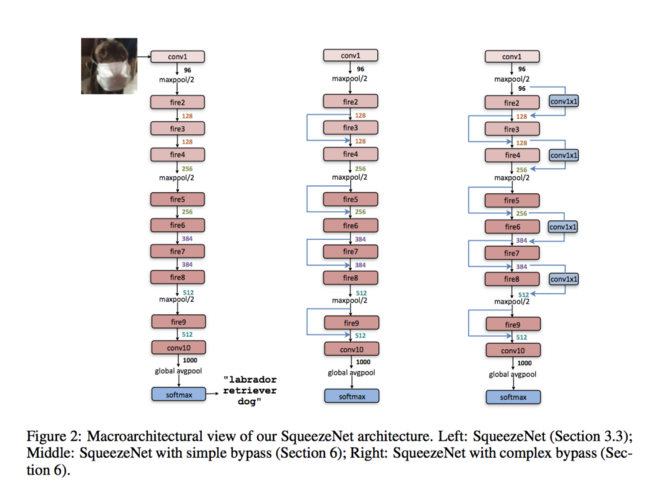
\includegraphics{squeezenet.png}
\caption{}
\end{figure}

    \subsubsection{javascript source code of SqueezeNet pulled from
github}\label{javascript-source-code-of-squeezenet-pulled-from-github}

    \begin{Verbatim}[commandchars=\\\{\}]
{\color{incolor}In [{\color{incolor} }]:} \PY{o}{/}\PY{o}{*}\PY{o}{*}
           \PY{o}{*} \PY{n}{Infer} \PY{n}{through} \PY{n}{SqueezeNet}\PY{p}{,} \PY{n}{assumes} \PY{n}{variables} \PY{n}{have} \PY{n}{been} \PY{n}{loaded}\PY{o}{.} \PY{n}{This} \PY{n}{does}
           \PY{o}{*} \PY{n}{standard} \PY{n}{ImageNet} \PY{n}{pre}\PY{o}{\PYZhy{}}\PY{n}{processing} \PY{n}{before} \PY{n}{inferring} \PY{n}{through} \PY{n}{the} \PY{n}{model}\PY{o}{.} \PY{n}{This}
           \PY{o}{*} \PY{n}{method} \PY{n}{returns} \PY{n}{named} \PY{n}{activations} \PY{k}{as} \PY{n}{well} \PY{k}{as} \PY{n}{pre}\PY{o}{\PYZhy{}}\PY{n}{softmax} \PY{n}{logits}\PY{o}{.} \PY{n}{The} \PY{n}{user}
           \PY{o}{*} \PY{n}{needs} \PY{n}{to} \PY{n}{clean} \PY{n}{up} \PY{n}{namedActivations} \PY{n}{after} \PY{n}{inferring}\PY{o}{.}
           \PY{o}{*}
           \PY{o}{*} \PY{n+nd}{@param} \PY{n}{preprocessedInput} \PY{n}{preprocessed} \PY{n+nb}{input} \PY{n}{Array}\PY{o}{.}
           \PY{o}{*} \PY{n+nd}{@return} \PY{n}{Named} \PY{n}{activations} \PY{o+ow}{and} \PY{n}{the} \PY{n}{pre}\PY{o}{\PYZhy{}}\PY{n}{softmax} \PY{n}{logits}\PY{o}{.}
           \PY{o}{*}\PY{o}{/}
          \PY{n}{infer}\PY{p}{(}\PY{n}{preprocessedInput}\PY{p}{)} \PY{p}{\PYZob{}}
            \PY{n}{const} \PY{n}{namedActivations} \PY{o}{=} \PY{p}{\PYZob{}}\PY{p}{\PYZcb{}}\PY{p}{;}
        
            \PY{n}{const} \PY{n}{avgpool10} \PY{o}{=} \PY{n}{this}\PY{o}{.}\PY{n}{math}\PY{o}{.}\PY{n}{scope}\PY{p}{(}\PY{p}{(}\PY{n}{keep}\PY{p}{)} \PY{o}{=}\PY{o}{\PYZgt{}} \PY{p}{\PYZob{}}
              \PY{n}{const} \PY{n}{conv1} \PY{o}{=} \PY{n}{this}\PY{o}{.}\PY{n}{math}\PY{o}{.}\PY{n}{conv2d}\PY{p}{(}
                  \PY{n}{preprocessedInput}\PY{p}{,} \PY{n}{this}\PY{o}{.}\PY{n}{variables}\PY{p}{[}\PY{l+s+s1}{\PYZsq{}}\PY{l+s+s1}{conv1\PYZus{}W:0}\PY{l+s+s1}{\PYZsq{}}\PY{p}{]}\PY{p}{,}
                  \PY{n}{this}\PY{o}{.}\PY{n}{variables}\PY{p}{[}\PY{l+s+s1}{\PYZsq{}}\PY{l+s+s1}{conv1\PYZus{}b:0}\PY{l+s+s1}{\PYZsq{}}\PY{p}{]}\PY{p}{,} \PY{l+m+mi}{2}\PY{p}{,} \PY{l+m+mi}{0}\PY{p}{)}\PY{p}{;}
              \PY{n}{const} \PY{n}{conv1relu} \PY{o}{=} \PY{n}{keep}\PY{p}{(}\PY{n}{this}\PY{o}{.}\PY{n}{math}\PY{o}{.}\PY{n}{relu}\PY{p}{(}\PY{n}{conv1}\PY{p}{)}\PY{p}{)}\PY{p}{;}
        
              \PY{n}{namedActivations}\PY{p}{[}\PY{l+s+s1}{\PYZsq{}}\PY{l+s+s1}{conv\PYZus{}1}\PY{l+s+s1}{\PYZsq{}}\PY{p}{]} \PY{o}{=} \PY{n}{conv1relu}\PY{p}{;}
        
              \PY{n}{const} \PY{n}{pool1} \PY{o}{=} \PY{n}{keep}\PY{p}{(}\PY{n}{this}\PY{o}{.}\PY{n}{math}\PY{o}{.}\PY{n}{maxPool}\PY{p}{(}\PY{n}{conv1relu}\PY{p}{,} \PY{l+m+mi}{3}\PY{p}{,} \PY{l+m+mi}{2}\PY{p}{,} \PY{l+m+mi}{0}\PY{p}{)}\PY{p}{)}\PY{p}{;}
              \PY{n}{namedActivations}\PY{p}{[}\PY{l+s+s1}{\PYZsq{}}\PY{l+s+s1}{maxpool\PYZus{}1}\PY{l+s+s1}{\PYZsq{}}\PY{p}{]} \PY{o}{=} \PY{n}{pool1}\PY{p}{;}
        
              \PY{n}{const} \PY{n}{fire2} \PY{o}{=} \PY{n}{keep}\PY{p}{(}\PY{n}{this}\PY{o}{.}\PY{n}{fireModule}\PY{p}{(}\PY{n}{pool1}\PY{p}{,} \PY{l+m+mi}{2}\PY{p}{)}\PY{p}{)}\PY{p}{;}
              \PY{n}{namedActivations}\PY{p}{[}\PY{l+s+s1}{\PYZsq{}}\PY{l+s+s1}{fire2}\PY{l+s+s1}{\PYZsq{}}\PY{p}{]} \PY{o}{=} \PY{n}{fire2}\PY{p}{;}
        
              \PY{n}{const} \PY{n}{fire3} \PY{o}{=} \PY{n}{keep}\PY{p}{(}\PY{n}{this}\PY{o}{.}\PY{n}{fireModule}\PY{p}{(}\PY{n}{fire2}\PY{p}{,} \PY{l+m+mi}{3}\PY{p}{)}\PY{p}{)}\PY{p}{;}
              \PY{n}{namedActivations}\PY{p}{[}\PY{l+s+s1}{\PYZsq{}}\PY{l+s+s1}{fire3}\PY{l+s+s1}{\PYZsq{}}\PY{p}{]} \PY{o}{=} \PY{n}{fire3}\PY{p}{;}
        
              \PY{o}{/}\PY{o}{/} \PY{n}{Because} \PY{n}{we} \PY{n}{don}\PY{l+s+s1}{\PYZsq{}}\PY{l+s+s1}{t have uneven padding yet, manually pad the ndarray on}
              \PY{o}{/}\PY{o}{/} \PY{n}{the} \PY{n}{right}\PY{o}{.}
              \PY{n}{const} \PY{n}{fire3Reshape2d} \PY{o}{=}
                  \PY{n}{fire3}\PY{o}{.}\PY{n}{as2D}\PY{p}{(}\PY{n}{fire3}\PY{o}{.}\PY{n}{shape}\PY{p}{[}\PY{l+m+mi}{0}\PY{p}{]}\PY{p}{,} \PY{n}{fire3}\PY{o}{.}\PY{n}{shape}\PY{p}{[}\PY{l+m+mi}{1}\PY{p}{]} \PY{o}{*} \PY{n}{fire3}\PY{o}{.}\PY{n}{shape}\PY{p}{[}\PY{l+m+mi}{2}\PY{p}{]}\PY{p}{)}\PY{p}{;}
              \PY{n}{const} \PY{n}{fire3Sliced2d} \PY{o}{=} \PY{n}{this}\PY{o}{.}\PY{n}{math}\PY{o}{.}\PY{n}{slice2D}\PY{p}{(}
                  \PY{n}{fire3Reshape2d}\PY{p}{,} \PY{p}{[}\PY{l+m+mi}{0}\PY{p}{,} \PY{l+m+mi}{0}\PY{p}{]}\PY{p}{,}
                  \PY{p}{[}\PY{n}{fire3}\PY{o}{.}\PY{n}{shape}\PY{p}{[}\PY{l+m+mi}{0}\PY{p}{]} \PY{o}{\PYZhy{}} \PY{l+m+mi}{1}\PY{p}{,} \PY{p}{(}\PY{n}{fire3}\PY{o}{.}\PY{n}{shape}\PY{p}{[}\PY{l+m+mi}{1}\PY{p}{]} \PY{o}{\PYZhy{}} \PY{l+m+mi}{1}\PY{p}{)} \PY{o}{*} \PY{n}{fire3}\PY{o}{.}\PY{n}{shape}\PY{p}{[}\PY{l+m+mi}{2}\PY{p}{]}\PY{p}{]}\PY{p}{)}\PY{p}{;}
              \PY{n}{const} \PY{n}{fire3Sliced} \PY{o}{=} \PY{n}{fire3Sliced2d}\PY{o}{.}\PY{n}{as3D}\PY{p}{(}
                  \PY{n}{fire3}\PY{o}{.}\PY{n}{shape}\PY{p}{[}\PY{l+m+mi}{0}\PY{p}{]} \PY{o}{\PYZhy{}} \PY{l+m+mi}{1}\PY{p}{,} \PY{n}{fire3}\PY{o}{.}\PY{n}{shape}\PY{p}{[}\PY{l+m+mi}{1}\PY{p}{]} \PY{o}{\PYZhy{}} \PY{l+m+mi}{1}\PY{p}{,} \PY{n}{fire3}\PY{o}{.}\PY{n}{shape}\PY{p}{[}\PY{l+m+mi}{2}\PY{p}{]}\PY{p}{)}\PY{p}{;}
              \PY{n}{const} \PY{n}{pool2} \PY{o}{=} \PY{n}{keep}\PY{p}{(}\PY{n}{this}\PY{o}{.}\PY{n}{math}\PY{o}{.}\PY{n}{maxPool}\PY{p}{(}\PY{n}{fire3Sliced}\PY{p}{,} \PY{l+m+mi}{3}\PY{p}{,} \PY{l+m+mi}{2}\PY{p}{,} \PY{l+m+mi}{0}\PY{p}{)}\PY{p}{)}\PY{p}{;}
              \PY{n}{namedActivations}\PY{p}{[}\PY{l+s+s1}{\PYZsq{}}\PY{l+s+s1}{maxpool\PYZus{}2}\PY{l+s+s1}{\PYZsq{}}\PY{p}{]} \PY{o}{=} \PY{n}{pool2}\PY{p}{;}
        
              \PY{n}{const} \PY{n}{fire4} \PY{o}{=} \PY{n}{keep}\PY{p}{(}\PY{n}{this}\PY{o}{.}\PY{n}{fireModule}\PY{p}{(}\PY{n}{pool2}\PY{p}{,} \PY{l+m+mi}{4}\PY{p}{)}\PY{p}{)}\PY{p}{;}
              \PY{n}{namedActivations}\PY{p}{[}\PY{l+s+s1}{\PYZsq{}}\PY{l+s+s1}{fire4}\PY{l+s+s1}{\PYZsq{}}\PY{p}{]} \PY{o}{=} \PY{n}{fire4}\PY{p}{;}
        
              \PY{n}{const} \PY{n}{fire5} \PY{o}{=} \PY{n}{keep}\PY{p}{(}\PY{n}{this}\PY{o}{.}\PY{n}{fireModule}\PY{p}{(}\PY{n}{fire4}\PY{p}{,} \PY{l+m+mi}{5}\PY{p}{)}\PY{p}{)}\PY{p}{;}
              \PY{n}{namedActivations}\PY{p}{[}\PY{l+s+s1}{\PYZsq{}}\PY{l+s+s1}{fire5}\PY{l+s+s1}{\PYZsq{}}\PY{p}{]} \PY{o}{=} \PY{n}{fire5}\PY{p}{;}
        
              \PY{n}{const} \PY{n}{pool3} \PY{o}{=} \PY{n}{keep}\PY{p}{(}\PY{n}{this}\PY{o}{.}\PY{n}{math}\PY{o}{.}\PY{n}{maxPool}\PY{p}{(}\PY{n}{fire5}\PY{p}{,} \PY{l+m+mi}{3}\PY{p}{,} \PY{l+m+mi}{2}\PY{p}{,} \PY{l+m+mi}{0}\PY{p}{)}\PY{p}{)}\PY{p}{;}
              \PY{n}{namedActivations}\PY{p}{[}\PY{l+s+s1}{\PYZsq{}}\PY{l+s+s1}{maxpool\PYZus{}3}\PY{l+s+s1}{\PYZsq{}}\PY{p}{]} \PY{o}{=} \PY{n}{pool3}\PY{p}{;}
        
              \PY{n}{const} \PY{n}{fire6} \PY{o}{=} \PY{n}{keep}\PY{p}{(}\PY{n}{this}\PY{o}{.}\PY{n}{fireModule}\PY{p}{(}\PY{n}{pool3}\PY{p}{,} \PY{l+m+mi}{6}\PY{p}{)}\PY{p}{)}\PY{p}{;}
              \PY{n}{namedActivations}\PY{p}{[}\PY{l+s+s1}{\PYZsq{}}\PY{l+s+s1}{fire6}\PY{l+s+s1}{\PYZsq{}}\PY{p}{]} \PY{o}{=} \PY{n}{fire6}\PY{p}{;}
        
              \PY{n}{const} \PY{n}{fire7} \PY{o}{=} \PY{n}{keep}\PY{p}{(}\PY{n}{this}\PY{o}{.}\PY{n}{fireModule}\PY{p}{(}\PY{n}{fire6}\PY{p}{,} \PY{l+m+mi}{7}\PY{p}{)}\PY{p}{)}\PY{p}{;}
              \PY{n}{namedActivations}\PY{p}{[}\PY{l+s+s1}{\PYZsq{}}\PY{l+s+s1}{fire7}\PY{l+s+s1}{\PYZsq{}}\PY{p}{]} \PY{o}{=} \PY{n}{fire7}\PY{p}{;}
        
              \PY{n}{const} \PY{n}{fire8} \PY{o}{=} \PY{n}{keep}\PY{p}{(}\PY{n}{this}\PY{o}{.}\PY{n}{fireModule}\PY{p}{(}\PY{n}{fire7}\PY{p}{,} \PY{l+m+mi}{8}\PY{p}{)}\PY{p}{)}\PY{p}{;}
              \PY{n}{namedActivations}\PY{p}{[}\PY{l+s+s1}{\PYZsq{}}\PY{l+s+s1}{fire8}\PY{l+s+s1}{\PYZsq{}}\PY{p}{]} \PY{o}{=} \PY{n}{fire8}\PY{p}{;}
        
              \PY{n}{const} \PY{n}{fire9} \PY{o}{=} \PY{n}{keep}\PY{p}{(}\PY{n}{this}\PY{o}{.}\PY{n}{fireModule}\PY{p}{(}\PY{n}{fire8}\PY{p}{,} \PY{l+m+mi}{9}\PY{p}{)}\PY{p}{)}\PY{p}{;}
              \PY{n}{namedActivations}\PY{p}{[}\PY{l+s+s1}{\PYZsq{}}\PY{l+s+s1}{fire9}\PY{l+s+s1}{\PYZsq{}}\PY{p}{]} \PY{o}{=} \PY{n}{fire9}\PY{p}{;}
        
              \PY{n}{const} \PY{n}{conv10} \PY{o}{=} \PY{n}{keep}\PY{p}{(}\PY{n}{this}\PY{o}{.}\PY{n}{math}\PY{o}{.}\PY{n}{conv2d}\PY{p}{(}
                  \PY{n}{fire9}\PY{p}{,} \PY{n}{this}\PY{o}{.}\PY{n}{variables}\PY{p}{[}\PY{l+s+s1}{\PYZsq{}}\PY{l+s+s1}{conv10\PYZus{}W:0}\PY{l+s+s1}{\PYZsq{}}\PY{p}{]}\PY{p}{,}
                  \PY{n}{this}\PY{o}{.}\PY{n}{variables}\PY{p}{[}\PY{l+s+s1}{\PYZsq{}}\PY{l+s+s1}{conv10\PYZus{}b:0}\PY{l+s+s1}{\PYZsq{}}\PY{p}{]}\PY{p}{,} \PY{l+m+mi}{1}\PY{p}{,} \PY{l+m+mi}{0}\PY{p}{)}\PY{p}{)}\PY{p}{;}
              \PY{n}{namedActivations}\PY{p}{[}\PY{l+s+s1}{\PYZsq{}}\PY{l+s+s1}{conv10}\PY{l+s+s1}{\PYZsq{}}\PY{p}{]} \PY{o}{=} \PY{n}{conv10}\PY{p}{;}
        
              \PY{k}{return} \PY{n}{this}\PY{o}{.}\PY{n}{math}\PY{o}{.}\PY{n}{avgPool}\PY{p}{(}\PY{n}{conv10}\PY{p}{,} \PY{n}{conv10}\PY{o}{.}\PY{n}{shape}\PY{p}{[}\PY{l+m+mi}{0}\PY{p}{]}\PY{p}{,} \PY{l+m+mi}{1}\PY{p}{,} \PY{l+m+mi}{0}\PY{p}{)}\PY{o}{.}\PY{n}{as1D}\PY{p}{(}\PY{p}{)}\PY{p}{;}
            \PY{p}{\PYZcb{}}\PY{p}{)}\PY{p}{;}
        
            \PY{k}{return} \PY{p}{\PYZob{}}\PY{n}{namedActivations}\PY{p}{,} \PY{n}{logits}\PY{p}{:} \PY{n}{avgpool10}\PY{p}{\PYZcb{}}\PY{p}{;}
          \PY{p}{\PYZcb{}}
        
          \PY{n}{fireModule}\PY{p}{(}\PY{n+nb}{input}\PY{p}{,} \PY{n}{fireId}\PY{p}{)} \PY{p}{\PYZob{}}
            \PY{n}{const} \PY{n}{y1} \PY{o}{=} \PY{n}{this}\PY{o}{.}\PY{n}{math}\PY{o}{.}\PY{n}{conv2d}\PY{p}{(}
                \PY{n+nb}{input}\PY{p}{,} \PY{n}{this}\PY{o}{.}\PY{n}{variables}\PY{p}{[}\PY{l+s+s1}{\PYZsq{}}\PY{l+s+s1}{fire}\PY{l+s+s1}{\PYZsq{}} \PY{o}{+} \PY{n}{fireId} \PY{o}{+} \PY{l+s+s1}{\PYZsq{}}\PY{l+s+s1}{/squeeze1x1\PYZus{}W:0}\PY{l+s+s1}{\PYZsq{}}\PY{p}{]}\PY{p}{,}
                \PY{n}{this}\PY{o}{.}\PY{n}{variables}\PY{p}{[}\PY{l+s+s1}{\PYZsq{}}\PY{l+s+s1}{fire}\PY{l+s+s1}{\PYZsq{}} \PY{o}{+} \PY{n}{fireId} \PY{o}{+} \PY{l+s+s1}{\PYZsq{}}\PY{l+s+s1}{/squeeze1x1\PYZus{}b:0}\PY{l+s+s1}{\PYZsq{}}\PY{p}{]}\PY{p}{,} \PY{l+m+mi}{1}\PY{p}{,} \PY{l+m+mi}{0}\PY{p}{)}\PY{p}{;}
            \PY{n}{const} \PY{n}{y2} \PY{o}{=} \PY{n}{this}\PY{o}{.}\PY{n}{math}\PY{o}{.}\PY{n}{relu}\PY{p}{(}\PY{n}{y1}\PY{p}{)}\PY{p}{;}
            \PY{n}{const} \PY{n}{left1} \PY{o}{=} \PY{n}{this}\PY{o}{.}\PY{n}{math}\PY{o}{.}\PY{n}{conv2d}\PY{p}{(}
                \PY{n}{y2}\PY{p}{,} \PY{n}{this}\PY{o}{.}\PY{n}{variables}\PY{p}{[}\PY{l+s+s1}{\PYZsq{}}\PY{l+s+s1}{fire}\PY{l+s+s1}{\PYZsq{}} \PY{o}{+} \PY{n}{fireId} \PY{o}{+} \PY{l+s+s1}{\PYZsq{}}\PY{l+s+s1}{/expand1x1\PYZus{}W:0}\PY{l+s+s1}{\PYZsq{}}\PY{p}{]}\PY{p}{,}
                \PY{n}{this}\PY{o}{.}\PY{n}{variables}\PY{p}{[}\PY{l+s+s1}{\PYZsq{}}\PY{l+s+s1}{fire}\PY{l+s+s1}{\PYZsq{}} \PY{o}{+} \PY{n}{fireId} \PY{o}{+} \PY{l+s+s1}{\PYZsq{}}\PY{l+s+s1}{/expand1x1\PYZus{}b:0}\PY{l+s+s1}{\PYZsq{}}\PY{p}{]}\PY{p}{,} \PY{l+m+mi}{1}\PY{p}{,} \PY{l+m+mi}{0}\PY{p}{)}\PY{p}{;}
            \PY{n}{const} \PY{n}{left2} \PY{o}{=} \PY{n}{this}\PY{o}{.}\PY{n}{math}\PY{o}{.}\PY{n}{relu}\PY{p}{(}\PY{n}{left1}\PY{p}{)}\PY{p}{;}
        
            \PY{n}{const} \PY{n}{right1} \PY{o}{=} \PY{n}{this}\PY{o}{.}\PY{n}{math}\PY{o}{.}\PY{n}{conv2d}\PY{p}{(}
                \PY{n}{y2}\PY{p}{,} \PY{n}{this}\PY{o}{.}\PY{n}{variables}\PY{p}{[}\PY{l+s+s1}{\PYZsq{}}\PY{l+s+s1}{fire}\PY{l+s+s1}{\PYZsq{}} \PY{o}{+} \PY{n}{fireId} \PY{o}{+} \PY{l+s+s1}{\PYZsq{}}\PY{l+s+s1}{/expand3x3\PYZus{}W:0}\PY{l+s+s1}{\PYZsq{}}\PY{p}{]}\PY{p}{,}
                \PY{n}{this}\PY{o}{.}\PY{n}{variables}\PY{p}{[}\PY{l+s+s1}{\PYZsq{}}\PY{l+s+s1}{fire}\PY{l+s+s1}{\PYZsq{}} \PY{o}{+} \PY{n}{fireId} \PY{o}{+} \PY{l+s+s1}{\PYZsq{}}\PY{l+s+s1}{/expand3x3\PYZus{}b:0}\PY{l+s+s1}{\PYZsq{}}\PY{p}{]}\PY{p}{,} \PY{l+m+mi}{1}\PY{p}{,} \PY{l+m+mi}{1}\PY{p}{)}\PY{p}{;}
            \PY{n}{const} \PY{n}{right2} \PY{o}{=} \PY{n}{this}\PY{o}{.}\PY{n}{math}\PY{o}{.}\PY{n}{relu}\PY{p}{(}\PY{n}{right1}\PY{p}{)}\PY{p}{;}
        
            \PY{k}{return} \PY{n}{this}\PY{o}{.}\PY{n}{math}\PY{o}{.}\PY{n}{concat3D}\PY{p}{(}\PY{n}{left2}\PY{p}{,} \PY{n}{right2}\PY{p}{,} \PY{l+m+mi}{2}\PY{p}{)}\PY{p}{;}
          \PY{p}{\PYZcb{}}
        
        \PY{n}{export} \PY{n}{default} \PY{n}{SqueezeNet}\PY{p}{;}
\end{Verbatim}


    \subsubsection{the tensorflow version of SqueezeNet model from cs231n
Stanford}\label{the-tensorflow-version-of-squeezenet-model-from-cs231n-stanford}

    \begin{Verbatim}[commandchars=\\\{\}]
{\color{incolor}In [{\color{incolor} }]:} \PY{k+kn}{import} \PY{n+nn}{tensorflow} \PY{k}{as} \PY{n+nn}{tf}
        
        \PY{n}{NUM\PYZus{}CLASSES} \PY{o}{=} \PY{l+m+mi}{1000}
        \PY{k}{def} \PY{n+nf}{fire\PYZus{}module}\PY{p}{(}\PY{n}{x}\PY{p}{,}\PY{n}{inp}\PY{p}{,}\PY{n}{sp}\PY{p}{,}\PY{n}{e11p}\PY{p}{,}\PY{n}{e33p}\PY{p}{)}\PY{p}{:}
            \PY{k}{with} \PY{n}{tf}\PY{o}{.}\PY{n}{variable\PYZus{}scope}\PY{p}{(}\PY{l+s+s2}{\PYZdq{}}\PY{l+s+s2}{fire}\PY{l+s+s2}{\PYZdq{}}\PY{p}{)}\PY{p}{:}
                \PY{k}{with} \PY{n}{tf}\PY{o}{.}\PY{n}{variable\PYZus{}scope}\PY{p}{(}\PY{l+s+s2}{\PYZdq{}}\PY{l+s+s2}{squeeze}\PY{l+s+s2}{\PYZdq{}}\PY{p}{)}\PY{p}{:}
                    \PY{n}{W} \PY{o}{=} \PY{n}{tf}\PY{o}{.}\PY{n}{get\PYZus{}variable}\PY{p}{(}\PY{l+s+s2}{\PYZdq{}}\PY{l+s+s2}{weights}\PY{l+s+s2}{\PYZdq{}}\PY{p}{,}\PY{n}{shape}\PY{o}{=}\PY{p}{[}\PY{l+m+mi}{1}\PY{p}{,}\PY{l+m+mi}{1}\PY{p}{,}\PY{n}{inp}\PY{p}{,}\PY{n}{sp}\PY{p}{]}\PY{p}{)}
                    \PY{n}{b} \PY{o}{=} \PY{n}{tf}\PY{o}{.}\PY{n}{get\PYZus{}variable}\PY{p}{(}\PY{l+s+s2}{\PYZdq{}}\PY{l+s+s2}{bias}\PY{l+s+s2}{\PYZdq{}}\PY{p}{,}\PY{n}{shape}\PY{o}{=}\PY{p}{[}\PY{n}{sp}\PY{p}{]}\PY{p}{)}
                    \PY{n}{s} \PY{o}{=} \PY{n}{tf}\PY{o}{.}\PY{n}{nn}\PY{o}{.}\PY{n}{conv2d}\PY{p}{(}\PY{n}{x}\PY{p}{,}\PY{n}{W}\PY{p}{,}\PY{p}{[}\PY{l+m+mi}{1}\PY{p}{,}\PY{l+m+mi}{1}\PY{p}{,}\PY{l+m+mi}{1}\PY{p}{,}\PY{l+m+mi}{1}\PY{p}{]}\PY{p}{,}\PY{l+s+s2}{\PYZdq{}}\PY{l+s+s2}{VALID}\PY{l+s+s2}{\PYZdq{}}\PY{p}{)}\PY{o}{+}\PY{n}{b}
                    \PY{n}{s} \PY{o}{=} \PY{n}{tf}\PY{o}{.}\PY{n}{nn}\PY{o}{.}\PY{n}{relu}\PY{p}{(}\PY{n}{s}\PY{p}{)}
                \PY{k}{with} \PY{n}{tf}\PY{o}{.}\PY{n}{variable\PYZus{}scope}\PY{p}{(}\PY{l+s+s2}{\PYZdq{}}\PY{l+s+s2}{e11}\PY{l+s+s2}{\PYZdq{}}\PY{p}{)}\PY{p}{:}
                    \PY{n}{W} \PY{o}{=} \PY{n}{tf}\PY{o}{.}\PY{n}{get\PYZus{}variable}\PY{p}{(}\PY{l+s+s2}{\PYZdq{}}\PY{l+s+s2}{weights}\PY{l+s+s2}{\PYZdq{}}\PY{p}{,}\PY{n}{shape}\PY{o}{=}\PY{p}{[}\PY{l+m+mi}{1}\PY{p}{,}\PY{l+m+mi}{1}\PY{p}{,}\PY{n}{sp}\PY{p}{,}\PY{n}{e11p}\PY{p}{]}\PY{p}{)}
                    \PY{n}{b} \PY{o}{=} \PY{n}{tf}\PY{o}{.}\PY{n}{get\PYZus{}variable}\PY{p}{(}\PY{l+s+s2}{\PYZdq{}}\PY{l+s+s2}{bias}\PY{l+s+s2}{\PYZdq{}}\PY{p}{,}\PY{n}{shape}\PY{o}{=}\PY{p}{[}\PY{n}{e11p}\PY{p}{]}\PY{p}{)}
                    \PY{n}{e11} \PY{o}{=} \PY{n}{tf}\PY{o}{.}\PY{n}{nn}\PY{o}{.}\PY{n}{conv2d}\PY{p}{(}\PY{n}{s}\PY{p}{,}\PY{n}{W}\PY{p}{,}\PY{p}{[}\PY{l+m+mi}{1}\PY{p}{,}\PY{l+m+mi}{1}\PY{p}{,}\PY{l+m+mi}{1}\PY{p}{,}\PY{l+m+mi}{1}\PY{p}{]}\PY{p}{,}\PY{l+s+s2}{\PYZdq{}}\PY{l+s+s2}{VALID}\PY{l+s+s2}{\PYZdq{}}\PY{p}{)}\PY{o}{+}\PY{n}{b}
                    \PY{n}{e11} \PY{o}{=} \PY{n}{tf}\PY{o}{.}\PY{n}{nn}\PY{o}{.}\PY{n}{relu}\PY{p}{(}\PY{n}{e11}\PY{p}{)}
                \PY{k}{with} \PY{n}{tf}\PY{o}{.}\PY{n}{variable\PYZus{}scope}\PY{p}{(}\PY{l+s+s2}{\PYZdq{}}\PY{l+s+s2}{e33}\PY{l+s+s2}{\PYZdq{}}\PY{p}{)}\PY{p}{:}
                    \PY{n}{W} \PY{o}{=} \PY{n}{tf}\PY{o}{.}\PY{n}{get\PYZus{}variable}\PY{p}{(}\PY{l+s+s2}{\PYZdq{}}\PY{l+s+s2}{weights}\PY{l+s+s2}{\PYZdq{}}\PY{p}{,}\PY{n}{shape}\PY{o}{=}\PY{p}{[}\PY{l+m+mi}{3}\PY{p}{,}\PY{l+m+mi}{3}\PY{p}{,}\PY{n}{sp}\PY{p}{,}\PY{n}{e33p}\PY{p}{]}\PY{p}{)}
                    \PY{n}{b} \PY{o}{=} \PY{n}{tf}\PY{o}{.}\PY{n}{get\PYZus{}variable}\PY{p}{(}\PY{l+s+s2}{\PYZdq{}}\PY{l+s+s2}{bias}\PY{l+s+s2}{\PYZdq{}}\PY{p}{,}\PY{n}{shape}\PY{o}{=}\PY{p}{[}\PY{n}{e33p}\PY{p}{]}\PY{p}{)}
                    \PY{n}{e33} \PY{o}{=} \PY{n}{tf}\PY{o}{.}\PY{n}{nn}\PY{o}{.}\PY{n}{conv2d}\PY{p}{(}\PY{n}{s}\PY{p}{,}\PY{n}{W}\PY{p}{,}\PY{p}{[}\PY{l+m+mi}{1}\PY{p}{,}\PY{l+m+mi}{1}\PY{p}{,}\PY{l+m+mi}{1}\PY{p}{,}\PY{l+m+mi}{1}\PY{p}{]}\PY{p}{,}\PY{l+s+s2}{\PYZdq{}}\PY{l+s+s2}{SAME}\PY{l+s+s2}{\PYZdq{}}\PY{p}{)}\PY{o}{+}\PY{n}{b}
                    \PY{n}{e33} \PY{o}{=} \PY{n}{tf}\PY{o}{.}\PY{n}{nn}\PY{o}{.}\PY{n}{relu}\PY{p}{(}\PY{n}{e33}\PY{p}{)}
                \PY{k}{return} \PY{n}{tf}\PY{o}{.}\PY{n}{concat}\PY{p}{(}\PY{p}{[}\PY{n}{e11}\PY{p}{,}\PY{n}{e33}\PY{p}{]}\PY{p}{,}\PY{l+m+mi}{3}\PY{p}{)}
        
        \PY{k}{class} \PY{n+nc}{SqueezeNet}\PY{p}{(}\PY{n+nb}{object}\PY{p}{)}\PY{p}{:}
            \PY{k}{def} \PY{n+nf}{extract\PYZus{}features}\PY{p}{(}\PY{n+nb+bp}{self}\PY{p}{,} \PY{n+nb}{input}\PY{o}{=}\PY{k+kc}{None}\PY{p}{,} \PY{n}{reuse}\PY{o}{=}\PY{k+kc}{True}\PY{p}{)}\PY{p}{:}
                \PY{k}{if} \PY{n+nb}{input} \PY{o+ow}{is} \PY{k+kc}{None}\PY{p}{:}
                    \PY{n+nb}{input} \PY{o}{=} \PY{n+nb+bp}{self}\PY{o}{.}\PY{n}{image}
                \PY{n}{x} \PY{o}{=} \PY{n+nb}{input}
                \PY{n}{layers} \PY{o}{=} \PY{p}{[}\PY{p}{]}
                \PY{k}{with} \PY{n}{tf}\PY{o}{.}\PY{n}{variable\PYZus{}scope}\PY{p}{(}\PY{l+s+s1}{\PYZsq{}}\PY{l+s+s1}{features}\PY{l+s+s1}{\PYZsq{}}\PY{p}{,} \PY{n}{reuse}\PY{o}{=}\PY{n}{reuse}\PY{p}{)}\PY{p}{:}
                    \PY{k}{with} \PY{n}{tf}\PY{o}{.}\PY{n}{variable\PYZus{}scope}\PY{p}{(}\PY{l+s+s1}{\PYZsq{}}\PY{l+s+s1}{layer0}\PY{l+s+s1}{\PYZsq{}}\PY{p}{)}\PY{p}{:}
                        \PY{n}{W} \PY{o}{=} \PY{n}{tf}\PY{o}{.}\PY{n}{get\PYZus{}variable}\PY{p}{(}\PY{l+s+s2}{\PYZdq{}}\PY{l+s+s2}{weights}\PY{l+s+s2}{\PYZdq{}}\PY{p}{,}\PY{n}{shape}\PY{o}{=}\PY{p}{[}\PY{l+m+mi}{3}\PY{p}{,}\PY{l+m+mi}{3}\PY{p}{,}\PY{l+m+mi}{3}\PY{p}{,}\PY{l+m+mi}{64}\PY{p}{]}\PY{p}{)}
                        \PY{n}{b} \PY{o}{=} \PY{n}{tf}\PY{o}{.}\PY{n}{get\PYZus{}variable}\PY{p}{(}\PY{l+s+s2}{\PYZdq{}}\PY{l+s+s2}{bias}\PY{l+s+s2}{\PYZdq{}}\PY{p}{,}\PY{n}{shape}\PY{o}{=}\PY{p}{[}\PY{l+m+mi}{64}\PY{p}{]}\PY{p}{)}
                        \PY{n}{x} \PY{o}{=} \PY{n}{tf}\PY{o}{.}\PY{n}{nn}\PY{o}{.}\PY{n}{conv2d}\PY{p}{(}\PY{n}{x}\PY{p}{,}\PY{n}{W}\PY{p}{,}\PY{p}{[}\PY{l+m+mi}{1}\PY{p}{,}\PY{l+m+mi}{2}\PY{p}{,}\PY{l+m+mi}{2}\PY{p}{,}\PY{l+m+mi}{1}\PY{p}{]}\PY{p}{,}\PY{l+s+s2}{\PYZdq{}}\PY{l+s+s2}{VALID}\PY{l+s+s2}{\PYZdq{}}\PY{p}{)}
                        \PY{n}{x} \PY{o}{=} \PY{n}{tf}\PY{o}{.}\PY{n}{nn}\PY{o}{.}\PY{n}{bias\PYZus{}add}\PY{p}{(}\PY{n}{x}\PY{p}{,}\PY{n}{b}\PY{p}{)}
                        \PY{n}{layers}\PY{o}{.}\PY{n}{append}\PY{p}{(}\PY{n}{x}\PY{p}{)}
                    \PY{k}{with} \PY{n}{tf}\PY{o}{.}\PY{n}{variable\PYZus{}scope}\PY{p}{(}\PY{l+s+s1}{\PYZsq{}}\PY{l+s+s1}{layer1}\PY{l+s+s1}{\PYZsq{}}\PY{p}{)}\PY{p}{:}
                        \PY{n}{x} \PY{o}{=} \PY{n}{tf}\PY{o}{.}\PY{n}{nn}\PY{o}{.}\PY{n}{relu}\PY{p}{(}\PY{n}{x}\PY{p}{)}
                        \PY{n}{layers}\PY{o}{.}\PY{n}{append}\PY{p}{(}\PY{n}{x}\PY{p}{)}
                    \PY{k}{with} \PY{n}{tf}\PY{o}{.}\PY{n}{variable\PYZus{}scope}\PY{p}{(}\PY{l+s+s1}{\PYZsq{}}\PY{l+s+s1}{layer2}\PY{l+s+s1}{\PYZsq{}}\PY{p}{)}\PY{p}{:}
                        \PY{n}{x} \PY{o}{=} \PY{n}{tf}\PY{o}{.}\PY{n}{nn}\PY{o}{.}\PY{n}{max\PYZus{}pool}\PY{p}{(}\PY{n}{x}\PY{p}{,}\PY{p}{[}\PY{l+m+mi}{1}\PY{p}{,}\PY{l+m+mi}{3}\PY{p}{,}\PY{l+m+mi}{3}\PY{p}{,}\PY{l+m+mi}{1}\PY{p}{]}\PY{p}{,}\PY{n}{strides}\PY{o}{=}\PY{p}{[}\PY{l+m+mi}{1}\PY{p}{,}\PY{l+m+mi}{2}\PY{p}{,}\PY{l+m+mi}{2}\PY{p}{,}\PY{l+m+mi}{1}\PY{p}{]}\PY{p}{,}\PY{n}{padding}\PY{o}{=}\PY{l+s+s1}{\PYZsq{}}\PY{l+s+s1}{VALID}\PY{l+s+s1}{\PYZsq{}}\PY{p}{)}
                        \PY{n}{layers}\PY{o}{.}\PY{n}{append}\PY{p}{(}\PY{n}{x}\PY{p}{)}
                    \PY{k}{with} \PY{n}{tf}\PY{o}{.}\PY{n}{variable\PYZus{}scope}\PY{p}{(}\PY{l+s+s1}{\PYZsq{}}\PY{l+s+s1}{layer3}\PY{l+s+s1}{\PYZsq{}}\PY{p}{)}\PY{p}{:}
                        \PY{n}{x} \PY{o}{=} \PY{n}{fire\PYZus{}module}\PY{p}{(}\PY{n}{x}\PY{p}{,}\PY{l+m+mi}{64}\PY{p}{,}\PY{l+m+mi}{16}\PY{p}{,}\PY{l+m+mi}{64}\PY{p}{,}\PY{l+m+mi}{64}\PY{p}{)}
                        \PY{n}{layers}\PY{o}{.}\PY{n}{append}\PY{p}{(}\PY{n}{x}\PY{p}{)}
                    \PY{k}{with} \PY{n}{tf}\PY{o}{.}\PY{n}{variable\PYZus{}scope}\PY{p}{(}\PY{l+s+s1}{\PYZsq{}}\PY{l+s+s1}{layer4}\PY{l+s+s1}{\PYZsq{}}\PY{p}{)}\PY{p}{:}
                        \PY{n}{x} \PY{o}{=} \PY{n}{fire\PYZus{}module}\PY{p}{(}\PY{n}{x}\PY{p}{,}\PY{l+m+mi}{128}\PY{p}{,}\PY{l+m+mi}{16}\PY{p}{,}\PY{l+m+mi}{64}\PY{p}{,}\PY{l+m+mi}{64}\PY{p}{)}
                        \PY{n}{layers}\PY{o}{.}\PY{n}{append}\PY{p}{(}\PY{n}{x}\PY{p}{)}
                    \PY{k}{with} \PY{n}{tf}\PY{o}{.}\PY{n}{variable\PYZus{}scope}\PY{p}{(}\PY{l+s+s1}{\PYZsq{}}\PY{l+s+s1}{layer5}\PY{l+s+s1}{\PYZsq{}}\PY{p}{)}\PY{p}{:}
                        \PY{n}{x} \PY{o}{=} \PY{n}{tf}\PY{o}{.}\PY{n}{nn}\PY{o}{.}\PY{n}{max\PYZus{}pool}\PY{p}{(}\PY{n}{x}\PY{p}{,}\PY{p}{[}\PY{l+m+mi}{1}\PY{p}{,}\PY{l+m+mi}{3}\PY{p}{,}\PY{l+m+mi}{3}\PY{p}{,}\PY{l+m+mi}{1}\PY{p}{]}\PY{p}{,}\PY{n}{strides}\PY{o}{=}\PY{p}{[}\PY{l+m+mi}{1}\PY{p}{,}\PY{l+m+mi}{2}\PY{p}{,}\PY{l+m+mi}{2}\PY{p}{,}\PY{l+m+mi}{1}\PY{p}{]}\PY{p}{,}\PY{n}{padding}\PY{o}{=}\PY{l+s+s1}{\PYZsq{}}\PY{l+s+s1}{VALID}\PY{l+s+s1}{\PYZsq{}}\PY{p}{)}
                        \PY{n}{layers}\PY{o}{.}\PY{n}{append}\PY{p}{(}\PY{n}{x}\PY{p}{)}
                    \PY{k}{with} \PY{n}{tf}\PY{o}{.}\PY{n}{variable\PYZus{}scope}\PY{p}{(}\PY{l+s+s1}{\PYZsq{}}\PY{l+s+s1}{layer6}\PY{l+s+s1}{\PYZsq{}}\PY{p}{)}\PY{p}{:}
                        \PY{n}{x} \PY{o}{=} \PY{n}{fire\PYZus{}module}\PY{p}{(}\PY{n}{x}\PY{p}{,}\PY{l+m+mi}{128}\PY{p}{,}\PY{l+m+mi}{32}\PY{p}{,}\PY{l+m+mi}{128}\PY{p}{,}\PY{l+m+mi}{128}\PY{p}{)}
                        \PY{n}{layers}\PY{o}{.}\PY{n}{append}\PY{p}{(}\PY{n}{x}\PY{p}{)}
                    \PY{k}{with} \PY{n}{tf}\PY{o}{.}\PY{n}{variable\PYZus{}scope}\PY{p}{(}\PY{l+s+s1}{\PYZsq{}}\PY{l+s+s1}{layer7}\PY{l+s+s1}{\PYZsq{}}\PY{p}{)}\PY{p}{:}
                        \PY{n}{x} \PY{o}{=} \PY{n}{fire\PYZus{}module}\PY{p}{(}\PY{n}{x}\PY{p}{,}\PY{l+m+mi}{256}\PY{p}{,}\PY{l+m+mi}{32}\PY{p}{,}\PY{l+m+mi}{128}\PY{p}{,}\PY{l+m+mi}{128}\PY{p}{)}
                        \PY{n}{layers}\PY{o}{.}\PY{n}{append}\PY{p}{(}\PY{n}{x}\PY{p}{)}
                    \PY{k}{with} \PY{n}{tf}\PY{o}{.}\PY{n}{variable\PYZus{}scope}\PY{p}{(}\PY{l+s+s1}{\PYZsq{}}\PY{l+s+s1}{layer8}\PY{l+s+s1}{\PYZsq{}}\PY{p}{)}\PY{p}{:}
                        \PY{n}{x} \PY{o}{=} \PY{n}{tf}\PY{o}{.}\PY{n}{nn}\PY{o}{.}\PY{n}{max\PYZus{}pool}\PY{p}{(}\PY{n}{x}\PY{p}{,}\PY{p}{[}\PY{l+m+mi}{1}\PY{p}{,}\PY{l+m+mi}{3}\PY{p}{,}\PY{l+m+mi}{3}\PY{p}{,}\PY{l+m+mi}{1}\PY{p}{]}\PY{p}{,}\PY{n}{strides}\PY{o}{=}\PY{p}{[}\PY{l+m+mi}{1}\PY{p}{,}\PY{l+m+mi}{2}\PY{p}{,}\PY{l+m+mi}{2}\PY{p}{,}\PY{l+m+mi}{1}\PY{p}{]}\PY{p}{,}\PY{n}{padding}\PY{o}{=}\PY{l+s+s1}{\PYZsq{}}\PY{l+s+s1}{VALID}\PY{l+s+s1}{\PYZsq{}}\PY{p}{)}
                        \PY{n}{layers}\PY{o}{.}\PY{n}{append}\PY{p}{(}\PY{n}{x}\PY{p}{)}
                    \PY{k}{with} \PY{n}{tf}\PY{o}{.}\PY{n}{variable\PYZus{}scope}\PY{p}{(}\PY{l+s+s1}{\PYZsq{}}\PY{l+s+s1}{layer9}\PY{l+s+s1}{\PYZsq{}}\PY{p}{)}\PY{p}{:}
                        \PY{n}{x} \PY{o}{=} \PY{n}{fire\PYZus{}module}\PY{p}{(}\PY{n}{x}\PY{p}{,}\PY{l+m+mi}{256}\PY{p}{,}\PY{l+m+mi}{48}\PY{p}{,}\PY{l+m+mi}{192}\PY{p}{,}\PY{l+m+mi}{192}\PY{p}{)}
                        \PY{n}{layers}\PY{o}{.}\PY{n}{append}\PY{p}{(}\PY{n}{x}\PY{p}{)}
                    \PY{k}{with} \PY{n}{tf}\PY{o}{.}\PY{n}{variable\PYZus{}scope}\PY{p}{(}\PY{l+s+s1}{\PYZsq{}}\PY{l+s+s1}{layer10}\PY{l+s+s1}{\PYZsq{}}\PY{p}{)}\PY{p}{:}
                        \PY{n}{x} \PY{o}{=} \PY{n}{fire\PYZus{}module}\PY{p}{(}\PY{n}{x}\PY{p}{,}\PY{l+m+mi}{384}\PY{p}{,}\PY{l+m+mi}{48}\PY{p}{,}\PY{l+m+mi}{192}\PY{p}{,}\PY{l+m+mi}{192}\PY{p}{)}
                        \PY{n}{layers}\PY{o}{.}\PY{n}{append}\PY{p}{(}\PY{n}{x}\PY{p}{)}
                    \PY{k}{with} \PY{n}{tf}\PY{o}{.}\PY{n}{variable\PYZus{}scope}\PY{p}{(}\PY{l+s+s1}{\PYZsq{}}\PY{l+s+s1}{layer11}\PY{l+s+s1}{\PYZsq{}}\PY{p}{)}\PY{p}{:}
                        \PY{n}{x} \PY{o}{=} \PY{n}{fire\PYZus{}module}\PY{p}{(}\PY{n}{x}\PY{p}{,}\PY{l+m+mi}{384}\PY{p}{,}\PY{l+m+mi}{64}\PY{p}{,}\PY{l+m+mi}{256}\PY{p}{,}\PY{l+m+mi}{256}\PY{p}{)}
                        \PY{n}{layers}\PY{o}{.}\PY{n}{append}\PY{p}{(}\PY{n}{x}\PY{p}{)}
                    \PY{k}{with} \PY{n}{tf}\PY{o}{.}\PY{n}{variable\PYZus{}scope}\PY{p}{(}\PY{l+s+s1}{\PYZsq{}}\PY{l+s+s1}{layer12}\PY{l+s+s1}{\PYZsq{}}\PY{p}{)}\PY{p}{:}
                        \PY{n}{x} \PY{o}{=} \PY{n}{fire\PYZus{}module}\PY{p}{(}\PY{n}{x}\PY{p}{,}\PY{l+m+mi}{512}\PY{p}{,}\PY{l+m+mi}{64}\PY{p}{,}\PY{l+m+mi}{256}\PY{p}{,}\PY{l+m+mi}{256}\PY{p}{)}
                        \PY{n}{layers}\PY{o}{.}\PY{n}{append}\PY{p}{(}\PY{n}{x}\PY{p}{)}
                \PY{k}{return} \PY{n}{layers}
        
            \PY{k}{def} \PY{n+nf}{\PYZus{}\PYZus{}init\PYZus{}\PYZus{}}\PY{p}{(}\PY{n+nb+bp}{self}\PY{p}{,} \PY{n}{save\PYZus{}path}\PY{o}{=}\PY{k+kc}{None}\PY{p}{,} \PY{n}{sess}\PY{o}{=}\PY{k+kc}{None}\PY{p}{)}\PY{p}{:}
                \PY{l+s+sd}{\PYZdq{}\PYZdq{}\PYZdq{}Create a SqueezeNet model.}
        \PY{l+s+sd}{        Inputs:}
        \PY{l+s+sd}{        \PYZhy{} save\PYZus{}path: path to TensorFlow checkpoint}
        \PY{l+s+sd}{        \PYZhy{} sess: TensorFlow session}
        \PY{l+s+sd}{        \PYZhy{} input: optional input to the model. If None, will use placeholder for input.}
        \PY{l+s+sd}{        \PYZdq{}\PYZdq{}\PYZdq{}}
                \PY{n+nb+bp}{self}\PY{o}{.}\PY{n}{image} \PY{o}{=} \PY{n}{tf}\PY{o}{.}\PY{n}{placeholder}\PY{p}{(}\PY{l+s+s1}{\PYZsq{}}\PY{l+s+s1}{float}\PY{l+s+s1}{\PYZsq{}}\PY{p}{,}\PY{n}{shape}\PY{o}{=}\PY{p}{[}\PY{k+kc}{None}\PY{p}{,}\PY{k+kc}{None}\PY{p}{,}\PY{k+kc}{None}\PY{p}{,}\PY{l+m+mi}{3}\PY{p}{]}\PY{p}{,}\PY{n}{name}\PY{o}{=}\PY{l+s+s1}{\PYZsq{}}\PY{l+s+s1}{input\PYZus{}image}\PY{l+s+s1}{\PYZsq{}}\PY{p}{)}
                \PY{n+nb+bp}{self}\PY{o}{.}\PY{n}{labels} \PY{o}{=} \PY{n}{tf}\PY{o}{.}\PY{n}{placeholder}\PY{p}{(}\PY{l+s+s1}{\PYZsq{}}\PY{l+s+s1}{int32}\PY{l+s+s1}{\PYZsq{}}\PY{p}{,} \PY{n}{shape}\PY{o}{=}\PY{p}{[}\PY{k+kc}{None}\PY{p}{]}\PY{p}{,} \PY{n}{name}\PY{o}{=}\PY{l+s+s1}{\PYZsq{}}\PY{l+s+s1}{labels}\PY{l+s+s1}{\PYZsq{}}\PY{p}{)}
                \PY{n+nb+bp}{self}\PY{o}{.}\PY{n}{layers} \PY{o}{=} \PY{p}{[}\PY{p}{]}
                \PY{n}{x} \PY{o}{=} \PY{n+nb+bp}{self}\PY{o}{.}\PY{n}{image}
                \PY{n+nb+bp}{self}\PY{o}{.}\PY{n}{layers} \PY{o}{=} \PY{n+nb+bp}{self}\PY{o}{.}\PY{n}{extract\PYZus{}features}\PY{p}{(}\PY{n}{x}\PY{p}{,} \PY{n}{reuse}\PY{o}{=}\PY{k+kc}{False}\PY{p}{)}
                \PY{n+nb+bp}{self}\PY{o}{.}\PY{n}{features} \PY{o}{=} \PY{n+nb+bp}{self}\PY{o}{.}\PY{n}{layers}\PY{p}{[}\PY{o}{\PYZhy{}}\PY{l+m+mi}{1}\PY{p}{]}
                \PY{k}{with} \PY{n}{tf}\PY{o}{.}\PY{n}{variable\PYZus{}scope}\PY{p}{(}\PY{l+s+s1}{\PYZsq{}}\PY{l+s+s1}{classifier}\PY{l+s+s1}{\PYZsq{}}\PY{p}{)}\PY{p}{:}
                    \PY{k}{with} \PY{n}{tf}\PY{o}{.}\PY{n}{variable\PYZus{}scope}\PY{p}{(}\PY{l+s+s1}{\PYZsq{}}\PY{l+s+s1}{layer0}\PY{l+s+s1}{\PYZsq{}}\PY{p}{)}\PY{p}{:}
                        \PY{n}{x} \PY{o}{=} \PY{n+nb+bp}{self}\PY{o}{.}\PY{n}{features}
                        \PY{n+nb+bp}{self}\PY{o}{.}\PY{n}{layers}\PY{o}{.}\PY{n}{append}\PY{p}{(}\PY{n}{x}\PY{p}{)}
                    \PY{k}{with} \PY{n}{tf}\PY{o}{.}\PY{n}{variable\PYZus{}scope}\PY{p}{(}\PY{l+s+s1}{\PYZsq{}}\PY{l+s+s1}{layer1}\PY{l+s+s1}{\PYZsq{}}\PY{p}{)}\PY{p}{:}
                        \PY{n}{W} \PY{o}{=} \PY{n}{tf}\PY{o}{.}\PY{n}{get\PYZus{}variable}\PY{p}{(}\PY{l+s+s2}{\PYZdq{}}\PY{l+s+s2}{weights}\PY{l+s+s2}{\PYZdq{}}\PY{p}{,}\PY{n}{shape}\PY{o}{=}\PY{p}{[}\PY{l+m+mi}{1}\PY{p}{,}\PY{l+m+mi}{1}\PY{p}{,}\PY{l+m+mi}{512}\PY{p}{,}\PY{l+m+mi}{1000}\PY{p}{]}\PY{p}{)}
                        \PY{n}{b} \PY{o}{=} \PY{n}{tf}\PY{o}{.}\PY{n}{get\PYZus{}variable}\PY{p}{(}\PY{l+s+s2}{\PYZdq{}}\PY{l+s+s2}{bias}\PY{l+s+s2}{\PYZdq{}}\PY{p}{,}\PY{n}{shape}\PY{o}{=}\PY{p}{[}\PY{l+m+mi}{1000}\PY{p}{]}\PY{p}{)}
                        \PY{n}{x} \PY{o}{=} \PY{n}{tf}\PY{o}{.}\PY{n}{nn}\PY{o}{.}\PY{n}{conv2d}\PY{p}{(}\PY{n}{x}\PY{p}{,}\PY{n}{W}\PY{p}{,}\PY{p}{[}\PY{l+m+mi}{1}\PY{p}{,}\PY{l+m+mi}{1}\PY{p}{,}\PY{l+m+mi}{1}\PY{p}{,}\PY{l+m+mi}{1}\PY{p}{]}\PY{p}{,}\PY{l+s+s2}{\PYZdq{}}\PY{l+s+s2}{VALID}\PY{l+s+s2}{\PYZdq{}}\PY{p}{)}
                        \PY{n}{x} \PY{o}{=} \PY{n}{tf}\PY{o}{.}\PY{n}{nn}\PY{o}{.}\PY{n}{bias\PYZus{}add}\PY{p}{(}\PY{n}{x}\PY{p}{,}\PY{n}{b}\PY{p}{)}
                        \PY{n+nb+bp}{self}\PY{o}{.}\PY{n}{layers}\PY{o}{.}\PY{n}{append}\PY{p}{(}\PY{n}{x}\PY{p}{)}
                    \PY{k}{with} \PY{n}{tf}\PY{o}{.}\PY{n}{variable\PYZus{}scope}\PY{p}{(}\PY{l+s+s1}{\PYZsq{}}\PY{l+s+s1}{layer2}\PY{l+s+s1}{\PYZsq{}}\PY{p}{)}\PY{p}{:}
                        \PY{n}{x} \PY{o}{=} \PY{n}{tf}\PY{o}{.}\PY{n}{nn}\PY{o}{.}\PY{n}{relu}\PY{p}{(}\PY{n}{x}\PY{p}{)}
                        \PY{n+nb+bp}{self}\PY{o}{.}\PY{n}{layers}\PY{o}{.}\PY{n}{append}\PY{p}{(}\PY{n}{x}\PY{p}{)}
                    \PY{k}{with} \PY{n}{tf}\PY{o}{.}\PY{n}{variable\PYZus{}scope}\PY{p}{(}\PY{l+s+s1}{\PYZsq{}}\PY{l+s+s1}{layer3}\PY{l+s+s1}{\PYZsq{}}\PY{p}{)}\PY{p}{:}
                        \PY{n}{x} \PY{o}{=} \PY{n}{tf}\PY{o}{.}\PY{n}{nn}\PY{o}{.}\PY{n}{avg\PYZus{}pool}\PY{p}{(}\PY{n}{x}\PY{p}{,}\PY{p}{[}\PY{l+m+mi}{1}\PY{p}{,}\PY{l+m+mi}{13}\PY{p}{,}\PY{l+m+mi}{13}\PY{p}{,}\PY{l+m+mi}{1}\PY{p}{]}\PY{p}{,}\PY{n}{strides}\PY{o}{=}\PY{p}{[}\PY{l+m+mi}{1}\PY{p}{,}\PY{l+m+mi}{13}\PY{p}{,}\PY{l+m+mi}{13}\PY{p}{,}\PY{l+m+mi}{1}\PY{p}{]}\PY{p}{,}\PY{n}{padding}\PY{o}{=}\PY{l+s+s1}{\PYZsq{}}\PY{l+s+s1}{VALID}\PY{l+s+s1}{\PYZsq{}}\PY{p}{)}
                        \PY{n+nb+bp}{self}\PY{o}{.}\PY{n}{layers}\PY{o}{.}\PY{n}{append}\PY{p}{(}\PY{n}{x}\PY{p}{)}
                \PY{n+nb+bp}{self}\PY{o}{.}\PY{n}{classifier} \PY{o}{=} \PY{n}{tf}\PY{o}{.}\PY{n}{reshape}\PY{p}{(}\PY{n}{x}\PY{p}{,}\PY{p}{[}\PY{o}{\PYZhy{}}\PY{l+m+mi}{1}\PY{p}{,} \PY{n}{NUM\PYZus{}CLASSES}\PY{p}{]}\PY{p}{)}
\end{Verbatim}


    Other than the parameters like filter numbers, kernel weight, kernel
height, we can see that the structure pretty much remain the same. The
SqueezeNet used in Teachable Machine does not make much changes
regarding the its architecture. Except when it later feed the
pre-softmax logits into KNN:

    \begin{Verbatim}[commandchars=\\\{\}]
{\color{incolor}In [{\color{incolor} }]:} \PY{n}{const} \PY{n}{knn} \PY{o}{=} \PY{n}{this}\PY{o}{.}\PY{n}{math}\PY{o}{.}\PY{n}{scope}\PY{p}{(}\PY{p}{(}\PY{n}{keep}\PY{p}{)} \PY{o}{=}\PY{o}{\PYZgt{}} \PY{p}{\PYZob{}}
                \PY{n}{const} \PY{n}{frameLogits} \PY{o}{=} \PY{n}{this}\PY{o}{.}\PY{n}{captureFrameSqueezeNetLogits}\PY{p}{(}\PY{p}{)}\PY{p}{;}
        
                \PY{k}{if} \PY{p}{(}\PY{n}{this}\PY{o}{.}\PY{n}{trainLogitsMatrix} \PY{o}{==}\PY{o}{=} \PY{n}{null}\PY{p}{)} \PY{p}{\PYZob{}}
                  \PY{n}{let} \PY{n}{newTrainLogitsMatrix} \PY{o}{=} \PY{n}{null}\PY{p}{;}
        
                  \PY{k}{for} \PY{p}{(}\PY{n}{let} \PY{n}{index} \PY{o}{=} \PY{l+m+mi}{0}\PY{p}{;} \PY{n}{index} \PY{o}{\PYZlt{}} \PY{n}{CLASS\PYZus{}COUNT}\PY{p}{;} \PY{n}{index} \PY{o}{+}\PY{o}{=} \PY{l+m+mi}{1}\PY{p}{)} \PY{p}{\PYZob{}}
                    \PY{n}{newTrainLogitsMatrix} \PY{o}{=} \PY{n}{this}\PY{o}{.}\PY{n}{concat}\PY{p}{(}
                      \PY{n}{newTrainLogitsMatrix}\PY{p}{,} \PY{n}{this}\PY{o}{.}\PY{n}{trainClassLogitsMatrices}\PY{p}{[}\PY{n}{index}\PY{p}{]}\PY{p}{)}\PY{p}{;}
                  \PY{p}{\PYZcb{}}
        
                  \PY{n}{this}\PY{o}{.}\PY{n}{trainLogitsMatrix} \PY{o}{=} \PY{n}{keep}\PY{p}{(}\PY{n}{this}\PY{o}{.}\PY{n}{math}\PY{o}{.}\PY{n}{clone}\PY{p}{(}\PY{n}{newTrainLogitsMatrix}\PY{p}{)}\PY{p}{)}\PY{p}{;}
                \PY{p}{\PYZcb{}}
        
                \PY{k}{return} \PY{n}{this}\PY{o}{.}\PY{n}{math}\PY{o}{.}\PY{n}{matMul}\PY{p}{(}
                  \PY{n}{this}\PY{o}{.}\PY{n}{trainLogitsMatrix}\PY{o}{.}\PY{n}{as2D}\PY{p}{(}\PY{n}{numExamples}\PY{p}{,} \PY{l+m+mi}{1000}\PY{p}{)}\PY{p}{,}
                  \PY{n}{frameLogits}\PY{o}{.}\PY{n}{as2D}\PY{p}{(}\PY{l+m+mi}{1000}\PY{p}{,} \PY{l+m+mi}{1}\PY{p}{)}\PY{p}{)}\PY{o}{.}\PY{n}{as1D}\PY{p}{(}\PY{p}{)}\PY{p}{;}
              \PY{p}{\PYZcb{}}\PY{p}{)}\PY{p}{;}
        
              \PY{n}{const} \PY{n}{computeConfidences} \PY{o}{=} \PY{p}{(}\PY{p}{)} \PY{o}{=}\PY{o}{\PYZgt{}} \PY{p}{\PYZob{}}
                \PY{n}{const} \PY{n}{values} \PY{o}{=} \PY{n}{knn}\PY{o}{.}\PY{n}{getValues}\PY{p}{(}\PY{p}{)}\PY{p}{;}
                \PY{n}{const} \PY{n}{kVal} \PY{o}{=} \PY{n}{Math}\PY{o}{.}\PY{n}{min}\PY{p}{(}\PY{n}{TOPK}\PY{p}{,} \PY{n}{numExamples}\PY{p}{)}\PY{p}{;}
                \PY{n}{const} \PY{n}{topK} \PY{o}{=} \PY{n}{this}\PY{o}{.}\PY{n}{mathCPU}\PY{o}{.}\PY{n}{topK}\PY{p}{(}\PY{n}{knn}\PY{p}{,} \PY{n}{kVal}\PY{p}{)}\PY{p}{;}
                \PY{n}{knn}\PY{o}{.}\PY{n}{dispose}\PY{p}{(}\PY{p}{)}\PY{p}{;}
        
        \PY{n}{const} \PY{n}{indices} \PY{o}{=} \PY{n}{topK}\PY{o}{.}\PY{n}{indices}\PY{o}{.}\PY{n}{getValues}\PY{p}{(}\PY{p}{)}\PY{p}{;}
\end{Verbatim}



    % Add a bibliography block to the postdoc
    
    
    
    \end{document}
